% arara: xelatex: { shell: yes }
% arara: makeglossaries
% arara: bibtex
% arara: xelatex: { shell: yes }
% arara: xelatex: { shell: yes }


% options:
% thesis=B bachelor's thesis
% thesis=M master's thesis
% czech thesis in Czech language
% english thesis in English language
% hidelinks remove colour boxes around hyperlinks

\documentclass[thesis=M,english]{FITthesis}[2019/12/23]

%\usepackage[utf8]{inputenc} % LaTeX source encoded as UTF-8
% \usepackage[latin2]{inputenc} % LaTeX source encoded as ISO-8859-2
% \usepackage[cp1250]{inputenc} % LaTeX source encoded as Windows-1250

% \usepackage{subfig} %subfigures
% \usepackage{amsmath} %advanced maths
% \usepackage{amssymb} %additional math symbols

\usepackage{dirtree} %directory tree visualisation
\usepackage{xcolor}
\usepackage{array}

% list padding
\usepackage{enumitem}

\definecolor{LightGray}{gray}{0.9}

% list of acronyms
\usepackage[acronym,nonumberlist,toc,numberedsection=autolabel,nomain]{glossaries}
\iflanguage{czech}{\renewcommand*{\acronymname}{Seznam pou{\v z}it{\' y}ch zkratek}}{}
\makeglossaries

\newglossaryentry{nosql}{name={NoSQL},description={NoSQL is a term for a database that does not use a relational model to store data. \cite{noauthor_what_nodate-1}}}
\newacronym{acid}{ACID}{Atomicity, Consistency, Isolation, Durability}
\newacronym{sql}{SQL}{Structured Query Language}
\newacronym{orm}{ORM}{Object-Relational Mapper}
\newacronym{ogm}{OGM}{Object-Graph Mapper}
\newacronym{http}{HTTP}{Hypertext Transfer Protocol}
\newacronym{pojo}{POJO}{Plain Old Java Object}
\newacronym{poco}{POCO}{Plain Old CLR Object}
\newacronym{crud}{CRUD}{Create, Read, Update, Delete}
\newacronym{dto}{DTO}{Data Transfer Object}
\newacronym{jit}{JIT}{Just-In-Time}
\newacronym{ide}{IDE}{Integrated Development Environment}
\newacronym{cil}{CIL}{Common Intermediate Language}
\newacronym{clr}{CLR}{Common Language Runtime}
\newacronym{sdk}{SDK}{Software Development Kit}
\newacronym{cli}{CLI}{Command Line Interface}
\newacronym{rdbms}{RDBMS}{Relational Database Management System}
\newacronym{tdd}{TDD}{Test-Driven Development}
\newacronym{dic}{DIC}{Dependency Injection Container}
\newacronym{api}{API}{Application Programming Interface}
\newacronym{cicd}{CI/CD}{Continuous Integration/Continuous Delivery}

\newcommand\taskfile{thesis_assignment.pdf}

\newcommand{\code}[1]{\mbox{\texttt{#1}}}

% % % % % % % % % % % % % % % % % % % % % % % % % % % % % %
% EDIT THIS
% % % % % % % % % % % % % % % % % % % % % % % % % % % % % %

\department{Department of software engineering}
\title{ORM Library for Neo4j Graph Database in .NET Framework}
\authorGN{} %author's given name/names
\authorFN{Starý} %author's surname
\author{Tomáš} %author's name without academic degrees
\authorWithDegrees{Bc. Tomáš Starý} %author's name with academic degrees
\supervisor{Ing. Marek Skotnica}
\acknowledgements{THANKS (remove entirely in case you do not with to thank anyone)}
\abstractEN{Summarize the contents and contribution of your work in a few sentences in English language.}
\abstractCS{V n{\v e}kolika v{\v e}t{\' a}ch shr{\v n}te obsah a p{\v r}{\' i}nos t{\' e}to pr{\' a}ce v {\v c}esk{\' e}m jazyce.}
\placeForDeclarationOfAuthenticity{Prague}
\keywordsCS{Replace with comma-separated list of keywords in Czech.}
\keywordsEN{Replace with comma-separated list of keywords in English.}
\declarationOfAuthenticityOption{4} %select as appropriate, according to the desired license (integer 1-6)
\website{https://github.com/TomStary/masters-thesis} %optional thesis URL


\begin{document}

% \newacronym{CVUT}{{\v C}VUT}{{\v C}esk{\' e} vysok{\' e} u{\v c}en{\' i} technick{\' e} v Praze}
% \newacronym{FIT}{FIT}{Fakulta informa{\v c}n{\' i}ch technologi{\' i}}

% \setsecnumdepth{part}

\begin{introduction}

    \section{Graphs are everywhere}

    In today's world, everything is highly connected.
    Graphs are an easy way to describe and visualize these relations and can help to see connections we would not otherwise catch.

    We do not use graphs to store data in most of our applications today, mainly because the first applications were made to take paper forms into the digital world.
    To keep these paper forms in digital format, we use relational databases.

    Since then, relational databases have been the go-to for every developer when creating a new application.
    Using a relational database is helpful for several reasons, mainly because the development cost is lower than using new technologies, and everyone is familiar with this type of \acrshort{dbms}.
    However, the lower development price benefits are diminished in today's world by the numerous problems with using relational databases.
    For example, lengthy searches for specific highly connected data and more complex relations are the main reason why \Gls{nosql} databases have been gaining so many tractions for the last decade.

    The graph databases are made explicitly with relationships in mind.
    Every vertex can have its connection with another one or even itself.
    This kind of connection is not possible with a relational database where connecting two rows means creating a relationship between two tables.
    To help with the performance of finding highly connected data, users can define indexes in relational databases, but there is only so much he can do.
    Indexes can slow the whole system down, inserts will be longer, and the entire database will increase memory consumption.

    \subsection{What can graph databases offer?}

    Graph databases are no silver bullet, and they cannot solve all our problems.
    When designing a new piece of software, we should always ask ourselves what the best technologies for the situation we are trying to solve is.

    We have discussed the problem with highly connected data and long searches, but how does the graph database solve this issue?
    The key here is that we will sooner or later find out that with more data comes more time spent on the same select with a growing relational database.
    This behaviour is due to numerous reasons, but the main one is that we are bound to make more costly joins with more extensive tables.
    Our search will be over the same part of the graph with a graph database no matter what happens with the rest. Execution times should therefore be the same.

    \section{How to use graph databases with object-oriented languages?}

    In most applications that communicate with a database, developers use an \acrshort{orm} to create objects from the database.
    This is a widespread way to use databases, and it is effortless to use. It creates an abstraction between the object-oriented language and \acrshort{sql}.
    Thus developers do not need a deep knowledge of \acrshort{sql} to use it.

    \acrshort{orm}s are powerful, but they are used only with relational databases, which is understandable given that \acrshort{orm} stands for Object-Relational Mapper.
    If we would like to use a mapper between a graph database and an object-oriented language, we would call it an \acrfull{ogm}. These types of mappers are not as widespread as \acrshort{orm}s are.

    In this paper, we will go through the steps of creating the \acrshort{ogm} library for \CS.
    We will start by studying graph databases and their query languages, studying similar solutions, namely EntityFramework, and end with our design and implementation of the library with proper testing.

\end{introduction}


\chapter {State of the art of graph databases}

Before we start with this chapter, here is a definition of what graph databases are:
"Graph databases store information in graphs, very similarly as relation databases store information in tables and have relations between columns in tables,
graph databases store information in nodes and even on the edges, or as we should call them, relations." \cite{morgante_what_2021}

To better show the power of graph databases, we will show it on a real-world example compared to relational databases.
Social networks dominate today's internet content, and everyone wants to be connected with his or her friends and relatives.
In one of the social networks, we have people who can post their thoughts or opinions.
Other users can follow them to see their posts, and also they can like those posts.
We can identify two entities with relations between them.
In a relational database, it would look like this.

\begin{figure}[H]
    \centering
    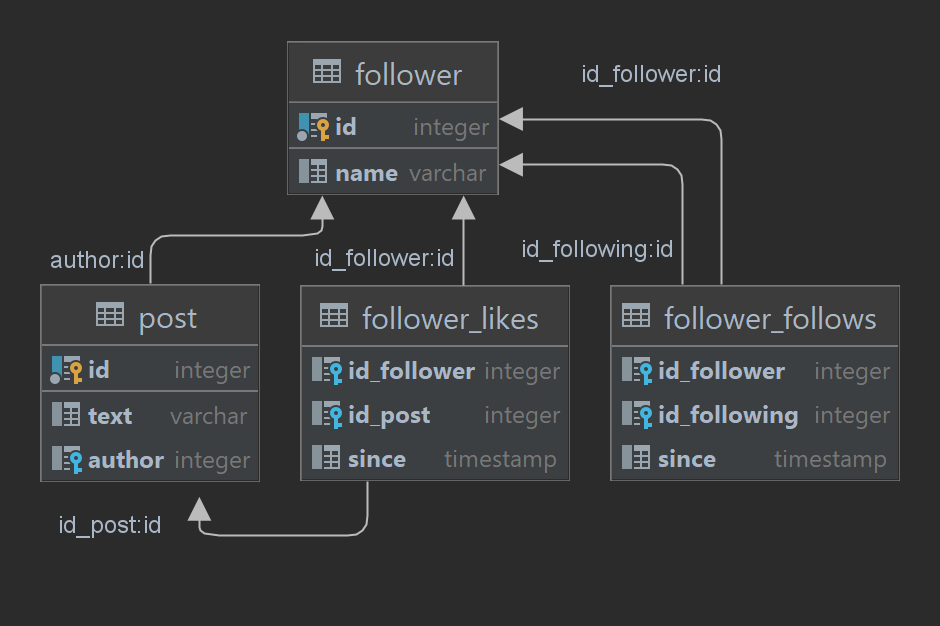
\includegraphics[width=0.7\textwidth]{content/relational-dbms-social-network.png}
    \caption{Relational database for social network}
\end{figure}

As we can see, we need four tables and five foreign keys to describe all relations between two identified entities.
This design can lead to costly joins to answer requests resulting from relationships between entities. For example, we could ask who follows followers who liked someone's post. The query for this example could then look like this:

\begin{listing}[H]
    \begin{minted}
 [
 frame=lines,
 framesep=2mm,
 baselinestretch=1.2,
 bgcolor=LightGray,
 linenos,
 breaklines
 ] {sql}
SELECT followers_of_followers_data.*
FROM post
JOIN follower_likes fl ON post.id = fl.id_post
JOIN follower followers_liked ON fl.id_follower = followers_liked.id
JOIN follower_follows followers_of_followers ON followers_liked.id = followers_of_followers.id_following
JOIN follower followers_of_followers_data ON followers_of_followers.id_follower = followers_of_followers_data.id
WHERE post.id = :post_id
ORDER BY followers_of_followers_data.name;
 \end{minted}
    \caption{SQL query for getting followers of followers who liked a post}
\end{listing}

From the query, we can see that it is barely readable and complex. However, the main problem is performance. The join operations will take more time even for the same request, with more data stored in tables.
Now, we compare the same problem solved using a graph database.

\begin{figure}[H]
    \centering
    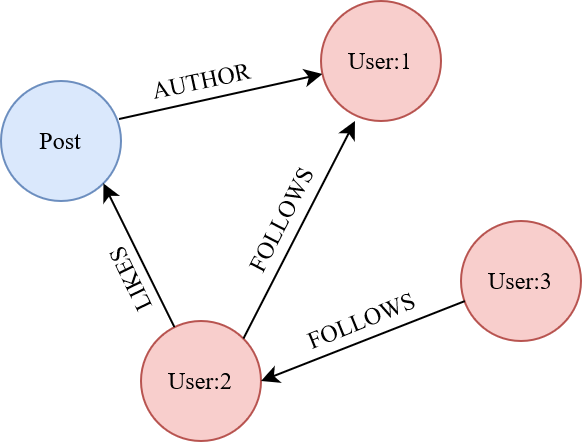
\includegraphics[width=0.8\textwidth]{content/graph_example.png}
    \caption{Graph database for social network}
\end{figure}

As we can see from the picture, each node has one relation or more to other nodes. Furthermore,
the answer to our question from the beginning is already visible if we remind ourselves:
who follows users that liked the post, we can then follow the path in the graph, and as we are going to discover in a moment,
the query to get this information also follows this path.

\begin{listing}[H]
    \begin{minted}
 [
 frame=lines,
 framesep=2mm,
 baselinestretch=1.2,
 bgcolor=LightGray,
 linenos,
 breaklines
 ] {cypher}
 MATCH (:Post {id: {post_id}})-[:LIKES]->(:User)-[:FOLLOWS]->(followers:User) RETURN (followers);
 \end{minted}
    \caption{Cypher query for getting followers of followers who liked a post}
\end{listing}

As promised, the query should not be hard to understand. It is just a quick example of how powerful graph databases can be.

This example was inspired by a blog post from Graham Cox, Introduction to Graph Databases. \cite{cox_introduction_2017}

\section {Native vs. Non-native graph databases}

When dealing with graph databases, we have to look at two main DBMS features: storage and processing.

Storage is how graphs are stored in memory. If the storage is optimized for graphs, like having related nodes close together, we talk about native graph storage when implementation uses other NoSQL storage. Then they are called non-native graph storage.

The second feature mentioned was processing, which refers to how graph databases process database operations. What is meant by that is how the database treats queries and how it handles storage. Native databases use Index-free adjacency for processing.
\cite{chao_graph_2018}

\textbf{Index-free adjacency}: "Native graphs take data that is logically connected via arcs or relationships and hard-wire the physical RAM addresses of these items into the node."
\cite{mccreary_neighborhood_2021} With this in mind, we can now see why graph databases are faster than other types of DBMS.
In traditional RDBMS, looking up a row in another table means that we have to pull an index table representing this relation and then find a path to row in said table.
This behavior leads to another problem in RDBMS because the database uses many indexes to keep data connected, which negatively impacts insert operations.

One more thing we should go through is how the graph database handles writes. Connected data requires strict data integrity.
Graph databases have to create or update nodes themselves and relationships; otherwise, this could result in a corrupted graph, which is almost impossible to fix.
The solution to this problem is to write fully \acrshort{acid}-compliant transactions, ensuring that the database will not become corrupted.
\cite{chao_graph_2018}

\section{Neo4j}

Neo4j is a graph database management system. It is developed by Neo4j, Inc., with its origin in Sweden. \cite{noauthor_company_nodate}
Neo4j is a native graph database, and it is also \acrshort{acid}-compliant. Given these properties, Neo4 uses its custom query language tailored explicitly for querying over graphs,
and its name is Cypher. \cite{noauthor_neo4j_nodate-2}

\section{Cypher}

\textit{Cypher} is a query language created by Neo4j initially for their graph database. Nowadays, it is possible to use Cypher on other graph databases, using "openCypher." \cite{noauthor_resources_nodate}

Its philosophy is to be easily read and understood by developers, database professionals, and business stakeholders.
Its ease of use derives from the fact that it is in accord with how we intuitively describe graphs using diagrams. \cite{robinson_graph_2015}

\subsection{Nodes}

To depict nodes in Cypher, we surround the node with parentheses, e.g., \texttt{(node)}. Parentheses were chosen because they look like circles,
a standard visual representation of nodes in the graph. \cite{noauthor_getting_nodate}

If we need to refer to the node, we can give it a variable like \texttt{(u)} for a user or \texttt{(p)} for a post.
In real-world queries, full names of variables should be used to understand the query better.

With variables, we mentioned the possibility to give a variable name to the nodes, but how can we distinguish two nodes from one to the other.
We can do this by assigning labels to each node. Labels are like tags, which specify certain entities in the graph. If we look back to our example of users and posts,
we can already identify the two labels we would use: \texttt{(p:Post)} and \texttt{(u:User)}.

Specifying labels also has another benefit. When not using labels in a query, the database has to look for all nodes, which can negatively impact the performance of the query.
\cite{noauthor_getting_nodate}

\subsection{Relationship representation}

Relationships between nodes are there to utilize the power of graph databases. They are represented in Cypher using an arrow \texttt{-->}
or \texttt{<--} between two nodes. Additional information, such as by which relationship type are two nodes connected and any properties of the relationship, can be placed in square brackets inside the arrow \texttt{((p:Post)-[:AUTHOR]->(u:User))}. \cite{noauthor_getting_nodate}

The direction of the relationship must be present only while creating the said relationship.
During the traversal of the graph, it is possible to omit the direction by using two dashes (like so: \texttt{--}).
This syntax can make queries more flexible and not force users to know in which directions are relationships stored in the database.

Like with nodes, variables can be used to refer to relationships. If we do not need to reference the relationship later,
we can leave any specification and use an anonymous relationship using two dashes.

\subsection{Nodes and relationship properties}

One thing that was not mentioned yet regarding nodes and relationships is properties. Each node and even each relationship can have one or more properties assigned to them.

Properties are name-value pairs providing additional detail. To represent them in the query, we place them in curly brackets. \cite{noauthor_getting_nodate}
Below is two examples of this usage, one for node and the other for relationship.

\begin{itemize}
    \item {Node property: \texttt{(u:User {nickname: 'mr. Incognito'})}}
    \item {Relationship property: \texttt{-[rel:AUTHOR {posted: 2022-02-05T12:12:20Z}]}}
\end{itemize}

\subsection{Querying with Cypher}

Cypher has few words reserved for specific actions called keywords like most other programming languages. \cite{noauthor_querying_nodate}
First, look at the two most common keywords:
\begin{itemize}
    \item {\texttt{MATCH}: This keyword is what searches for an existing node, relationship, label, property, or pattern in the database. \texttt{MATCH} does work similarly to the \texttt{SELECT} in \acrshort{sql}.}
    \item {\texttt{RETURN}: The \texttt{RETURN} keyword defines what values or results we want to retrieve from the database.
          It is used mainly in search queries as it is not required to be used during write procedures.
          \texttt{RETURN} does utilize the node and relationship variables. If we want to return any results from defined \texttt{MATCH},
          we must specify which nodes, relationships, properties, or patterns we want to return.}
\end{itemize}

\subsection{Create, update, and delete operations}

Besides queries, a proper database system must have methods to create, update or delete data.

The function \texttt{CREATE} is used to insert new data into a graph using Cypher language.
Using \texttt{CREATE}, we can create nodes, relationships, and also patterns. Below are some examples of how \texttt{CREATE} is used and the result. \cite{noauthor_updating_nodate}

\begin{listing}[H]
    \begin{minted}
 [
 frame=lines,
 framesep=2mm,
 baselinestretch=1.2,
 bgcolor=LightGray,
 linenos,
 breaklines
 ] {cypher}
 CREATE (u:User {nickname: "mr. Incognito"})
 RETURN u
 \end{minted}
    \caption{Create a new user with nickname}
\end{listing}

As we can see from examples, we can use the \texttt{RETURN} clause, but it is unnecessary in most cases.

In the following example, we will see \texttt{MATCH} being used before creating a relationship between two nodes.
If we used \texttt{CREATE} right away, we would introduce duplicities of both nodes.

\begin{listing}[H]
    \begin{minted}
 [
 frame=lines,
 framesep=2mm,
 baselinestretch=1.2,
 bgcolor=LightGray,
 linenos,
 breaklines
 ] {cypher}
 MATCH (u:User {nickname: "mr. Incognito"})
 MATCH (p:Post {title: "Hello, world!"})
 CREATE (u)<-[:AUTHOR]-(p)
 \end{minted}
    \caption{Create a new relationship between two nodes}
\end{listing}

There is another way to create this relationship, and we will look at it later in this chapter.

To update data in the database, Cypher uses a \texttt{SET} keyword, which can create or update node or relationship properties.

If we want to delete a node or relationship, we use the \texttt{DELETE} keyword in Cypher language.
This is similar to how \acrshort{sql} \texttt{DELETE} works, but with one exception. If a node is in a relationship
with another node, we cannot delete it because it would create an inconsistent graph, with a potential relationship pointing to nothing. \cite{noauthor_updating_nodate}

We could run two queries to delete the relationship and delete the node itself, but there is a more straightforward solution.
We can use \texttt{DETACH DELETE}, which does detach all relationships from the node before deleting it.

\section{\acrshort{orm}}
\acrshort{orm} stands for an object-relational mapper, which is based on the concept of object-relational mapping.
Object-relational mapping is the idea of writing queries using the object-oriented paradigm.
There are some limitations of what \acrshort{orm} can accomplish. Developers should always consider these limits before using an \acrshort{orm} framework. \cite{mario_hoyos_what_2018}

\noindent Pros:
\begin{itemize}
    \item There is no need to use a second language during software development, \acrshort{sql} is a powerful language, but most developers do not use it too often.
    \item \acrshort{orm} abstracts away from the database system.
    \item It can lead to better performance than writing queries by ourselves.
\end{itemize}
Cons:
\begin{itemize}
    \item If a developer is an \acrshort{sql} power user, he can write queries that will perform better.
    \item Developers have to learn how to use \acrshort{orm} properly.
    \item Developers still need to know how does \acrshort{orm} works under the hood.
\end{itemize}

Using the term \acrshort{orm} with relation to graph databases is not correct. The proper term would be \acrshort{ogm} (object-graph mapper),
but there are a few reasons why we are using \acrshort{orm} instead of \acrshort{ogm} in the name of this thesis. However, please make no mistake,
when discussing \acrshort{orm} involving graph databases, it is, in fact, \acrshort{ogm}.
The main reason is simple: \acrshort{orm} has been around for more than a decade, and developers are familiar with the concept and its challenges.

\section{Conclusion}

In this chapter, we introduced graph databases compared to relational databases. We compared the queries of both types of databases and their differences.
We also studied the differences between native and non-native databases.

The rest of this chapter was focused on Neo4j and Cypher language, where we introduced the basics of this language, like how are relationships and nodes defined,
and base keywords used in Cypher.

In the end, we also adequately introduced the concept of \acrshort{orm} and its relation to \acrshort{ogm}.


% \chapter{Architectures \& design patterns}

In this thesis, we will encounter a few architectures and design patterns. Before we do that, we should know what each of
them stands for. This chapter will go through the most notable patterns and describe them.

"Design Patterns are categorized mainly into three categories: Creational Design Pattern, Structural Design Pattern, and Behavioral
Design Pattern. These differ based on their level of detail, complexity, and scale of applicability to the entire system being designed." \cite{noauthor_classification_nodate}

\section{Creational design patterns}

As the name would suggest, Creational design patterns use abstraction for the instantiation process.
Using them makes a system independent of how its objects are created, composed, and represented. We can divide this pattern between
a class creational pattern, which uses inheritance to vary the class that's instantiated, and an object creational pattern, which will
delegate instantiation to another object. \cite{gamma_design_1995}

The main reason to use any of the creational design patterns is to help create an
abstraction layer for creating concrete instances of classes in a system.
This need comes with any system that is growing. Class inheritance may be enough at the start of the development,
but with a growing system comes a need to shift from class inheritance to delegation of instantiation to another object.
This is the time when creational design patterns come into play. These patterns give us much more flexibility
in what gets created, who creates it, how it gets created, and when.

\subsection{Abstract factory}

For an illustration, we will look at creating instances of different shapes.
We have got three shapes: triangle, square, pentagon. Each shape can be in different
variants like filled or with gradient background. The problem is how to abstract creating
each shape and its variant to match other objects of the same family. We also want to keep our
existing code intact, so we do not have to change our code repeatedly. \cite{gamma_design_1995}

To solve this problem with the abstract factory, we first declare interfaces for each distinct product of
the product family (e.g., triangle, square, pentagon). The next move is to declare the abstract factory, which is an interface with
a list of methods for all products that are part of the product family (for example, "createTriangle," "createSquare," "createPentagon").
These methods must return abstract types, which we declared at the beginning.

We create a separate factory class for product variants based on the abstract factory interface we declared for each of the variants.
We can call this implementation of the factory a concrete factory, which returns concrete products. In the client's code, we then accept the abstract
factory interface, giving us the ability to change the implementation of the concrete factory without the need to change the client's code.

One question is left unanswered, who creates the concrete factory instances? Usually, the application creates factories during
the initialization process; sometimes, these factories are part of the dependency injection container, but we will discuss this matter in another part of this chapter.

\subsection{Factory method}

Factory method provides an interface for creating objects in a superclass but allows subclasses to alter the type of created objects.
\cite{noauthor_factory_nodate} Using this solution, we will not use direct calls to the constructor in the application's code, but instead,
we will always call a defined method in our factory for a given class.

Imagine that we have an application that creates squares instances inside its code. As the application grows,
we encounter a new requirement to create another shape instead of a square. Each shape will have common methods.
If we continued to create objects inside the application's code, we would have to make a condition for each constructor invocation for shape.
Adding unnecessary complexity and this solution would be prone to errors.

Instead, we create a common interface for shapes. For this interface, we create a base factory (abstract class) with logic shared between final shapes.
Concrete factory is then used to define which product (shape in our case) is returned to the application's code.

The client's code using this pattern does not see a difference between the concrete product returned by various concrete subclasses.
It only sees the abstract interface that we declared.

\subsection{Builder pattern}

\chapter {State of the art EntityFramework and .NET}

If anyone wants to create \acrshort{orm} or \acrshort{ogm} for .NET in C\#, they should go through some principles that are used in
EntityFramework and .NET. This chapter will go through some of these principles with insight into the technologies used.

We will start with studying C\# and then .NET and LINQ, part of .NET. Then we will go through EntityFramework itself.

\section {C\#}
C\# is a general-purpose, type-safe, object-oriented programming language, the goal of which is programmer productivity.
To this end, the language balances simplicity, expressiveness,
and performance. \cite{albahari_c_2019}

Microsoft is developing and maintaining the C\# language. When writing this thesis, the current version of the C\# is C\#10.

The C\# code is statically compiled down to \acrlong{cil}. \acrshort{cil} cannot be run by itself on a machine.
\acrshort{cil} runtime or \acrfull{clr} must be used. Using \acrfull{jit} compilation, \acrshort{clr} reads \acrshort{cil} and translates \acrshort{cil} to native
code or sometimes called machine code. The machine's processor can then read machine code. Using \acrshort{cil} and \acrshort{clr} has benefits in running code
cross-platform without recompiling code for different processors, at the cost of some performance. \cite{rodenburg_code_2021}

\section {.NET}

.NET is a framework written for C\# and other languages such as F\# and
Visual Basic and Microsoft also develop them.
In their own words: ".NET is an open source developer
platform, created by Microsoft, for building many different types of applications." \cite{noauthor_what_nodate-2}

To compile a library or program with a .NET framework,
developers must first download and install a .NET \acrfull{sdk}.
.NET \acrfull{sdk} is either a standalone \acrfull{cli} tool or embedded inside an \acrshort{ide},
for example, in Visual Studio from Microsoft.

\subsection{Reflection}

The reflection pattern is used to access the class and its methods and fields. We can access the class and its methods and fields without knowing its implementation.
This feature has to be supported by the programming language itself. For example, C\# supports reflection and is widely used in many popular libraries.

Reflection works by scanning the program's implementations and creating metadata about the classes and methods.
This metadata is stored in the program's memory and made accessible at runtime.

For example, the following class:

\begin{listing}[H]
    \begin{minted}[
 frame=lines,
 framesep=2mm,
 baselinestretch=1.2,
 bgcolor=LightGray,
 linenos,
 breaklines
 ] {csharp}
 public class Person
 {
 [Key]
 public string Name { get; set; }
 public int Age { get; set; }
 }
\end{minted}
\end{listing}

If we would want to know if the class does contain a field with KeyAttribute annotation, we could use this next code to get the MemberInfo instance:

\begin{listing}[H]
    \begin{minted}[
 frame=lines,
 framesep=2mm,
 baselinestretch=1.2,
 bgcolor=LightGray,
 linenos,
 breaklines
 ] {csharp}
 public bool HasKeyAttribute(Type type)
 {
 var members = type.GetMembers();
 return members.Any(member => member.GetCustomAttributes().OfType<EndNodeAttribute>().Any());
 }
 \end{minted}
\end{listing}

We would use this code in cases where we do not know how an object is implemented.

\subsection {LINQ}

In the previous section, we used a method called \texttt{Any} to check if a collection contains an element. This method is part of a library in .NET called LINQ.
LINQ stands for Language Integrated Query, and it is a library that provides a set of methods that can be used to query objects.
We can filter, order, group, and transform data using this library.

LINQ is internally working as an expression tree, each command as an expression. The expression tree is immutable and evaluated at runtime, and developers
can use the tree to analyze and convert it to \acrshort{sql}, for example. To extend expression tree capabilities, LINQ provides an abstract class \texttt{ExpressionVisitor},
called for each expression combined with extension for \texttt{IQueryable<T>} and other tools.


With LINQ, we can write queries in a more readable way. These queries can then be translated to \acrshort{sql} queries, for example.
This feature is used in Entity Framework.

\section {Entity Framework Core}

With knowledge from previous sections of this chapter, we can now study Entity Framework.

When we are talking about Entity Framework, we are talking about their latest version of this framework, Entity Framework Core or EFCore, as it is known in the community.
This version was released for .NET Core 1.0, the first Microsoft version of .NET purposely built for multiplatform use.

To use Entity Framework, developers must add another dependency to their projects. This dependency is for Entity Framework and its called provider, which is used
to provide connection and translation capabilities for Entity Framework to work correctly over a specific database.

If we want to know how Entity Framework translates LINQ queries to SQL queries, we need to look at implementing any publicly available provider.
In a perfect world, we would use the documentation for how to do it, but there is no current documentation at the time of writing.

To study, we will choose a provider for the Postgresql database. There are two reasons for why this provider, the first one is the author's experience with these providers and the second one
is because a third party created this provider.

Complete code for this provider is available at GitHub server at this URL: \url{https://github.com/npgsql/efcore.pg}.

\subsection {Postgresql provider}

Studying both provider and Entity Framework Core, we get an idea of how it works. EF Core is creating a base functionality, like providing interfaces and abstract classes to scan
the expression tree for each query. It also provides interfaces for translators to translate the query to SQL. The provider is then implementing these interfaces and abstract classes.

As we already know, an expression tree is created from individual expressions. Each expression accepts visitors, which are used to generate \acrshort{sql}.
This expression tree is processed in
\linebreak\texttt{QueryCompilationContext}.

\subsection {\texttt{DbSet}}

An inseparable part of the Entity Framework Core is the \texttt{DbSet}. This class is used to query data from the database.
The Entity Framework creates it, and it is an implementation of \texttt{IQueryable<T>} interface. This interface is the backbone of LINQ.

With this abstract class, we can not only create queries to the database but also add or update entities to the change tracker.
Change tracker is then used for saving operation, where it is checked what was changed were made and then they are saved to the database using \texttt{DbContext.SaveChanges} method
or its asynchronous version \texttt{DbContext.SaveChangesAsync}.

\texttt{DbSet} implements methods in both synchronous and asynchronous versions. The main benefit of asynchronous versions is that they are not blocking the thread. They are using \texttt{Task} to run the code in the background. This is done by using \texttt{async} keyword.

One key aspect of queries not mentioned yet is that queries are generated using extension methods. Inside Entity Framework are declared extension methods that
extends \texttt{IQueryable<T>} interface and \text{Expression} abstract class. These extension methods are responsible for generating predicates which are then translated to the \acrshort{sql}.
To show these extensions, we will look at the example of implementation of \texttt{DbSet<T>.FindAsync} method.

\subsection{\texttt{FindAsync}}

Before going into the implementation, we need to define what this method does. It is used to find an entity by its primary key or keys.
If the key is not found, then it returns null, or to be more precise, it returns the default value of the object using keyword \texttt{default}.

\texttt{FindAsync} method does take 1 to n parameters of the type of object, and these parameters are key parameters of the entity we want to find, the entity,
which we want to find is given by the type used when declaring the \texttt{DbSet<T>} instance in \texttt{DbContext} either by declaring public property inside \texttt{DbContext}
or by using \texttt{DbContext.Set<T>} method.

Inside \texttt{FindAsync} is then called a method defined by \texttt{IEntityFinder} interface with name \texttt{FindAsync}.
The actual implementation is therefore hidden in the implementation of this implementation, which we can find inside the Entity Framework Core repository, which is available
on the GitHub server.

An instance of \texttt{EntityFinder} that implements \texttt{IEntityFinder} is created internally and also contains the cache for already tracked and mapped entities.
This cache is then checked to see if the entity we are trying to find is not already there. If it was the case, then the cached value is returned. Otherwise, a new query is created
using \texttt{FirstOrDefaultAsync} method which is \texttt{IQueryable<T>} extension method defined in the Entity Framework Core.

Queries are generally created by creating a custom expression tree, which is then translated to \acrshort{sql}.

\section {Summary}

\todo[inline]{TBD}



\chapter {Similar solutions}

\section{Neo4j-\acrshort{ogm}}

Neo4j company has already created an \acrshort{ogm} for their database. It supports dynamic objects and maps nodes and their relations into the domain model.
It is written in Java, but it should be a starting point when designing a similar library in the C\#.

\noindent Main features:
\begin{itemize}
    \item Object graph mapping of annotated node- and relationship-entities
    \item Neo4jSession for direct interaction with Neo4j
    \item Fast class metadata scanning
    \item Optimized management of data loading and change tracking for minimal data transfers
    \item Multiple transports: binary (bolt), \acrshort{http} and embedded
    \item Persistence lifecycle events
    \item Query result projection to data transfer objects (\acrshort{dto})
\end{itemize}

The following sections are information obtained from the official documentation of Neo4j-OGM for Java. \cite{noauthor_reference_nodate}

\subsection {Neo4j drivers}

There are three possible drivers to use, Bolt driver, \acrshort{http} driver, or embedded driver, which creates in-memory Neo4j instance.

Using a different driver in the development or test environment will not affect the production code. These drivers are interchangeable without the need for modification in queries.

\subsection {Entities}

This library offers us the possibility to define and shape entities and relationships. \texttt{@NodeEntity} annotation is used to declare that a \acrfull{pojo}
is indeed a node. This class must have one empty public constructor to allow the library to construct the objects.

Fields on the entity are by default mapped to properties of the node. Fields referencing other node entities (or collections thereof) are linked with relationships.

If we want to change fields name or other properties, we can use annotations like \texttt{@Property}, \texttt{@Id}, \texttt{@GeneratedValue}, or \texttt{@Relationship}. On the other hand,
if we want to not include a field in the node, we can use annotations \texttt{@Transient}.

\subsection {Relationships}

Every field of an entity that references one or more other node entities is backed by relationships in the graph. These relationships are managed by Neo4j-\acrshort{ogm} automatically.

If we want to specify relationship properties, like the direction of the relationship, the \texttt{@Relationship} annotation is used. The directions are either \texttt{INCOMING},
\texttt{OUTGOING}, or \texttt{UNDIRECTED}, where the last one ensures that the path between two node entities is navigable from either side.

Neo4j gives us the ability to define properties in relationships. Neo4j solves this using an entity (\acrshort{pojo}) with annotation \texttt{@RelationshipEntity}.

A String attribute called type is available on the \texttt{@RelationshipEntity} annotation to control the relationship type. Like the simple strategy for labeling node entities,
if this is not provided, then the class's name is used to derive the relationship type, although it is converted into \texttt{SNAKE\_CASE} to honor
the naming conventions of Neo4j relationships. \cite{noauthor_reference_nodate}

Inside the entity, we then define @StartNode and \texttt{@EndNode}. In referenced entities, we also define a reference to
the related entity and use @Relationship with type same as in \texttt{@RelationshipEntity}.

Below is an example of such usage:

\begin{listing}[!ht]
    \begin{minted}
    [
    frame=lines,
    framesep=2mm,
    baselinestretch=1.2,
    bgcolor=LightGray,
    linenos
    ] {java}
@NodeEntity
public class Actor {
    Long id;
    @Relationship(type="PLAYED_IN") private Role playedIn;
}

@RelationshipEntity(type = "PLAYED_IN")
public class Role {
    @Id @GeneratedValue   private Long relationshipId;
    @Property  private String title;
    @StartNode private Actor actor;
    @EndNode   private Movie movie;
}

@NodeEntity
public class Movie {
    private Long id;
    private String title;
}
    \end{minted}
    \caption{An example of entities with relationship as separate entity}
    \label{listing:1}
\end{listing}

\subsection {Indexes}

Annotations can define indexes. We already saw one of them, \texttt{@Id}, an annotation for the primary index.

But primary indexes are not the only type of index we can define in our models. We can also define indexes for other
properties using \texttt{@Index} annotation. We get an index with constraint if we use \texttt{@Index(unique=true)}.

This library also supports composite indexes and node constraints with \texttt{@CompositeIndex} and \texttt{@CompositeIndex(unique = true)}, respectively.

\texttt{@Required} is an existence constraint. "It is possible to annotate properties in both node entities and relationship entities. For node entities
the label of declaring class is used to create the constraint. For relationship entities the relationship type is used - such type must
be defined on leaf class." \cite{noauthor_reference_nodate}

The \acrshort{ogm} library can handle creating and managing indexes or constraints, but as stated in the documentation, this feature should be used only for development
and not in production. That is why this feature is, by default, turned off.


These are the available modes:
\begin{table}[H]
    \begin{center}
        \begin{tabularx}{\textwidth}{|c|p{0.83\textwidth}|}
            \hline
            node     & Default, nothing is done on the side of the OGM library.                                  \\
            \hline
            validate & This ensures that all constraints and indexes are in the database before starting up.     \\
            \hline
            assert   & This drops all indexes on startup and then creates only these defined by OGM annotations. \\
            \hline
            update   & Update indexes and constraints based on annotations.                                      \\
            \hline
            dump     & Dumps all indexes and constraints to a file.                                              \\
            \hline
        \end{tabularx}
        \caption{Available modes for indexes and constraints}
    \end{center}
\end{table}

\subsection{Sessions}
To interact with mapped entities, Neo4j-OGM requires a \texttt{Session}, which \texttt{SessionFactory} provides. Besides providing \texttt{Session}, \texttt{SessionFactory}
also setups up the object graph mapping metadata when constructed. That is then used across all \texttt{Session} objects created by \texttt{SessionFactory}.

Session keeps track of mapped entities, their changes, and changes between their relationships. Tracking is then used when saving or otherwise
working with mapped entities. When an entity is loaded by session, reloading this entity is then done from cache within the session.

To keep new data and not prolong sessions too much, session lifetime can be managed in code. Too long session lifetime
means that other users can change data, and too short a lifetime means costly save operations will be executed more often. There is a way
to force the session's cache to clear, but it is advised against it.

Cypher drives Neo4j-\acrshort{ogm} queries only. This means that only \acrfull{crud} operations are available. Documentation
suggests using server-side operations for more complex or performant graph traversals over the graph.
Nevertheless, Cypher should be powerful enough for most of the problems.

\subsection {Persisting entities}

Session allows to save, load, loadAll, and delete entities with transaction handling, and exception translation managed.
Persistence is performed through method save. This method then looks at underlying \texttt{MappingContext} and compares data loaded
from the database with the saved entity, creating appropriate Cypher queries to update the database based on differences.
Calling save is necessary to propagate changes because Neo4j-\acrshort{ogm} does not automatically commit changes.

The method has a second optional parameter: the depth, which can restrict how much depth the save will perform.
The default value is \texttt{-1}, which means saving every change in node and all reachable nodes from it into the database.
This approach is recommended because of possible inconsistencies that could happen.

\subsection {Loading entities}

Loading entities can be done using methods \texttt{session.loadxxx} or writing a custom Cypher query with methods \texttt{session.query} and \texttt{session.queryForObject}.
Like the depth for saving function, the load functions also have a depth.

Depth is there to determine how many depths of relatives will be loaded with query. The default behavior is to load the object's simple properties and neighbors.
This represents loading data using depth set to value 1. Depth is mainly helpful when loading deeper than broader parts of a graph. Depth also helps developers to
execute fewer load operations from the database.

When using load methods from the session, the session uses \texttt{LoadStrategy} to generate a \texttt{RETURN} clause. The default strategy is schema loading,
which uses entities metadata. The other is the path load strategy that uses paths from the root node. It is possible to change the strategy for a query using \texttt{Session.setStrategy}
or globally by calling \texttt{SessionFactory.setStrategy}.

\subsection{Transactions}

Neo4j uses transactions, which means queries can be executed only in transaction boundaries. Neo4j-\acrshort{ogm}
offers tools to manage transactions, but the developer does not have to use them because the session handles them independently but with the auto-commit transaction.


\chapter {Design of OGM library}

We should now have all information we need to propose our solution for OGM using the \CS language.
Before we start to analyze individual pieces of the library needed for its proper function, we need a list of requirements.

The solution should be able to:
\begin{itemize}
    \item {connect to a database}
    \item {map objects into graph structure}
    \item {map LINQ query into Cypher query}
    \item {execute a command in a database}
    \item {retrieve a result from the database}
    \item {map the result from the database into objects}
\end{itemize}

With these minimal requirements set, we can now go through them, analyze them, and propose individual solutions to them.

\section{Connect to a database}

Neo4j company has created a client for .NET that supports both bolt and neo4j URI schemes. \cite{noauthor_client_nodate} This driver is a standalone NuGet package that is publicly accessible and licensed under Apache 2.0 license. This means we can use this driver in our library as a dependency.

The application should handle the driver's lifecycle. During startup, the application should create an instance of the driver and then correctly destroy this instance on exit. The lifecycle will be managed by our library or by using DIC.

Before we create an instance of the driver, we need to pass the correct configuration for the driver. Configuration for the driver and session must be created and maintained. .NET does contain a configuration manager used with the linkage to dependency injection.

Here is visualisation of connections between components:

\begin{figure}[H]
    \centering
    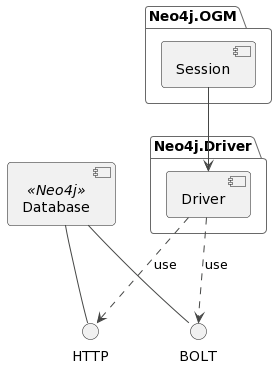
\includegraphics[width=0.4\textwidth]{content/components.png}
    \caption{Components diagram}
\end{figure}

\subsection{Conclusion}

We will use Neo4j's official driver for connection, but we need to encapsulate it into our library.
We need to create a configuration structure and configuration builder, which will then be used to create a connection to the database.

\section {Map objects into graph structure}

If we want to correctly translate queries from the object paradigm into Cypher, we need to know the graph structure described in our domain.

What we are trying to do is create metadata. To build metadata, we first need information, which assemblies contain models representing nodes and relationships in a graph. A developer must declare these assemblies as it is necessary to limit the scope that will be scanned using reflection.

The solutions we analyzed in the previous chapter are internally working very similarly. Both are scanning assemblies or packages on initialization (Java uses packages vs. \CS uses assemblies/namespaces), and we will borrow some of the features from these solutions into ours.
Developers of our library will need to define a set of assemblies. During the initialization of our library, we will scan these assemblies and create a metadata object with information about the user-defined graph.

\subsection {Annotations}

To create a metadata object, we need to identify and process nodes and relationships. We need to have a way for developers to describe each node and its relationship with all properties they would want to define, and which we also need to build the metadata object correctly.

We already have a solution to this problem, and Neo4j also uses it to solve the same issue. We will use annotations using attributes. Using these annotations, we can describe nodes and their relationships.

We will look for these annotations during initialization using reflection, which is well supported by \CS and .NET. With annotation, we can describe the graph and create the metadata object.

\subsection {Entity mapper}

Entity mapper should be able to map entities into statements that could then be translated into Cypher query. It should be able to use generated metadata correctly
to map both nodes and relationships.

For this purpose, we will define a interface \texttt{IEntityMapper}. This interface will contain
this list of public methods:

\begin{itemize}
    \item {\texttt{Map}: this method map an entity to a \texttt{ICompilerContext}}
    \item {\texttt{CompilerContext}: this method returns a current instance of\linebreak\texttt{ICompilerContext}}
\end{itemize}

In the picture \ref{fig:IEntityMapperClassDiagram} is class diagram with interfaces and also classes that implements these interfaces.
The interface \texttt{ICompilerContext} contains methods for controlling the context of mapped nodes and relationships. These methods
are used during mapping an entity in \texttt{IEntityMapper.Map} method to map an entity for Cypher query.

\begin{figure}[H]
    \centering
    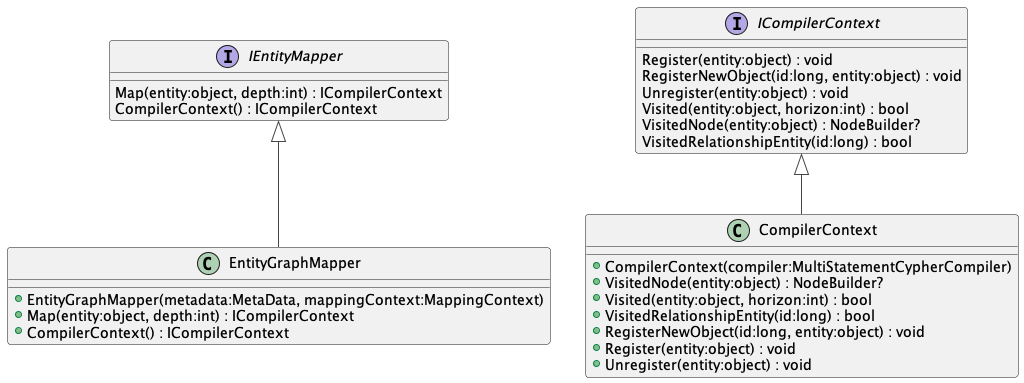
\includegraphics[width=0.8\textwidth]{content/entitymapper.png}
    \caption{\texttt{IEntityMapper} and \texttt{ICompilerContext} class diagrams}
    \label{fig:IEntityMapperClassDiagram}
\end{figure}

\section {Map LINQ query into Cypher query}

Mapping a LINQ query to a Cypher query is a bit more complicated. As we already know, any LINQ query is an expression tree used to process an IQueryable object.
We cannot map these expressions to a Cypher query because we do not know how to map the expression tree to a Cypher query. However, there is a way to transform the expression tree
into a Cypher query. We know this because Entity Framework does the same thing for SQL queries. We can illustrate the process of transformation using the state diagram
\ref{fig:querystate}.

\begin{figure}[H]
    \centering
    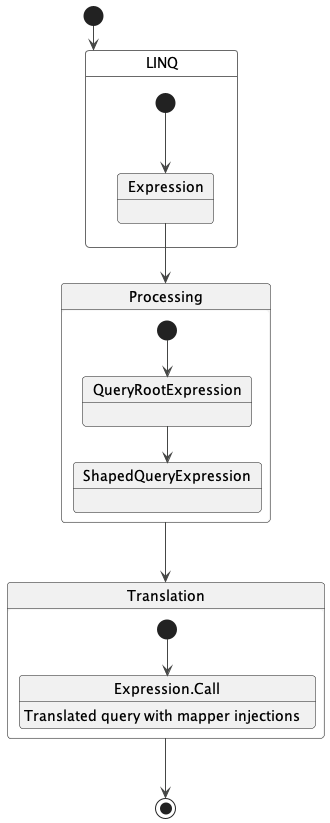
\includegraphics[width=0.5\textwidth]{content/Expression transformation.png}
    \caption{LINQ expression transformation}
    \label{fig:querystate}
\end{figure}

\subsection{\texttt{IQueryable} extension}

If we want to communicate with the database, the \texttt{IQueryable} instance must have a correct provider.
This provider must be able to transform the expression tree into a Cypher query and also execute the query asynchronously. We are going to extend \texttt{IQueryProvider} interface
with \texttt{IAsyncQueryProvider} interface which declares \texttt{IAsyncQueryProvider.ExecuteAsync<T>} method.

To set a correct provider we are going to define new class that implements \texttt{IQueryable<T>} interface called \texttt{DbSet<T>}.
The name of the class is the same as it is in Entity Framework. Besides implementing \texttt{IQueryable<T>} interface \texttt{DbSet<T>} class also implements
\texttt{IAsyncEnumerable<T>} interface. This interface is used to create an asynchronous enumerable object.

Inside the constructor of \texttt{DbSet<T>} class, we are going to set the correct provider as well as set an instance of \texttt{ISession}.
Because we need an instance of \texttt{ISession} we are going to declare a method inside this interface called
\texttt{ISession.Set<TEntity>} which will create a new instance
of \texttt{DbSet<T>}.

Because we are communicating with a database using asynchronous operations, we need to create extension methods for \texttt{DbSet<T>} which are also asynchronous.
For example, LINQ has method called \texttt{FirstOrDefault} which returns first element of \texttt{IQueryable<T>} or default value of type T. We are going to create
an extension of \texttt{IQueryable<T>} with method \texttt{FirstOrDefaultAsync}. This extension method will transform the expression tree into a Cypher query.

Inside this extension method, we will call providers\linebreak
\code{IAsyncQueryProvider.ExecuteAsync<T>} method. This is our entry point, from which we will start a translation
of the expression tree into a Cypher query.

For better visualisation, here \ref{fig:queryprovider} is class diagram of query provider and\linebreak\texttt{DbSet<T>} class.

\begin{figure}[H]
    \centering
    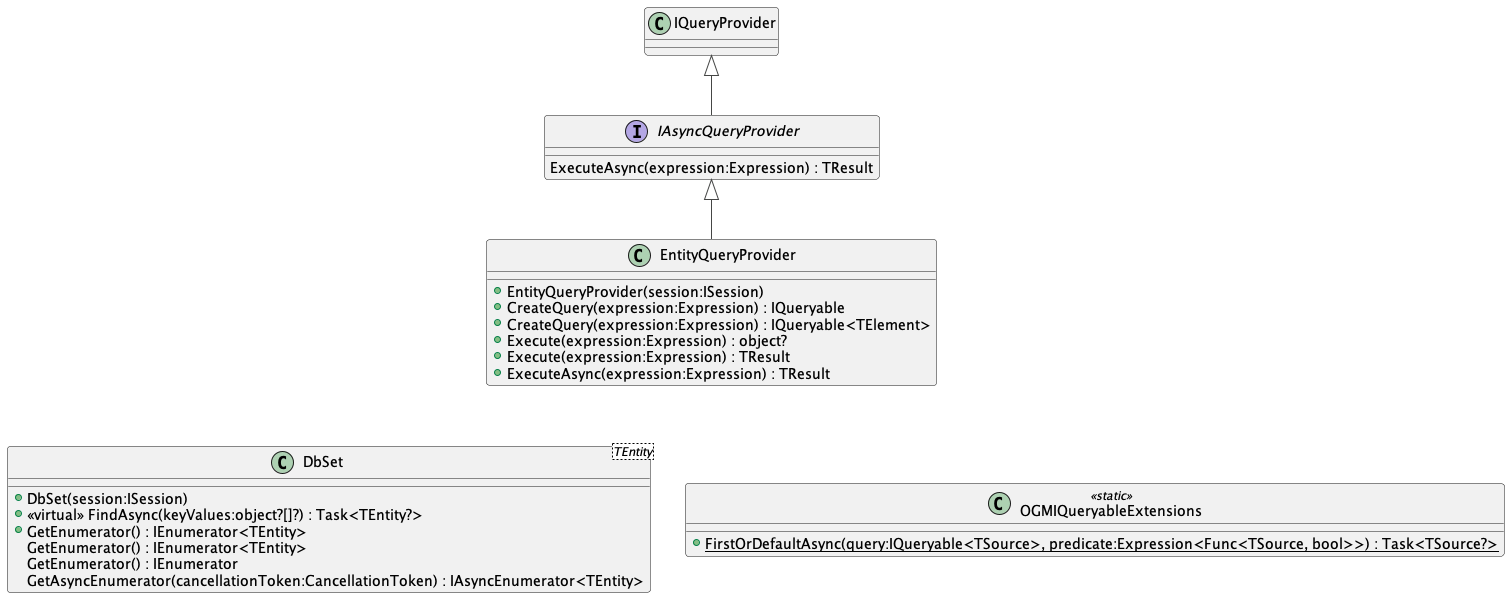
\includegraphics[width=0.9\textwidth]{content/QueryProvider.png}
    \caption{\texttt{IAsyncQueryProvider} and \texttt{DbSet<TEnity>} with extension class diagram}
    \label{fig:queryprovider}
\end{figure}

\subsection{Query compilation}

To best visualize the process of query compilation, we will use sequence
diagram \ref{fig:QueryCompilerSequence}. In this diagram, we can see how we will employ
the\linebreak\texttt{ExpressionVisitor} abstract class to visit the expression tree and, through the different steps, recreate it to the state which is needed to compile the Cypher query.

The result of this compilation will be a \texttt{Func<QueryContext, TResult>}, which is an object representing the function.
This function does both a query execution and enumerates a result from a database response.

In the sequence diagram \ref{fig:QueryCompilerSequence}, are three expression tree visitors, each serving different purpose. Using these visitors
gives us the ability to expand our library's capabilities easily. We would only need to create a new visitor who would comply with
the existing expression. We can also further expand the capabilities of defined visitors inside their implementation.

We should also introduce the concerns of each visitor. The first one that is used in the diagram is \texttt{ParameterExtractingExpressionVisitor},
which extracts parameters from the original expression. The next one is\linebreak\texttt{QueryableMethodTranslationExpressionVisitor}, this visitor will
be responsible for translating the original LINQ query into an expression tree that will be consisted of \texttt{CypherExpression} derivatives,
which will copy the Cypher language structure. The last visitor is\linebreak\texttt{ShapedQueryCompilinExpressionVisitor}, it is responsible
for taking a\linebreak\texttt{ShapedQueryExpression} and translating it into a \texttt{Expression.Call} expression, which can be then compiled into
the \texttt{Func<QueryContext, TResult>} object.

\begin{figure}[H]
    \centering
    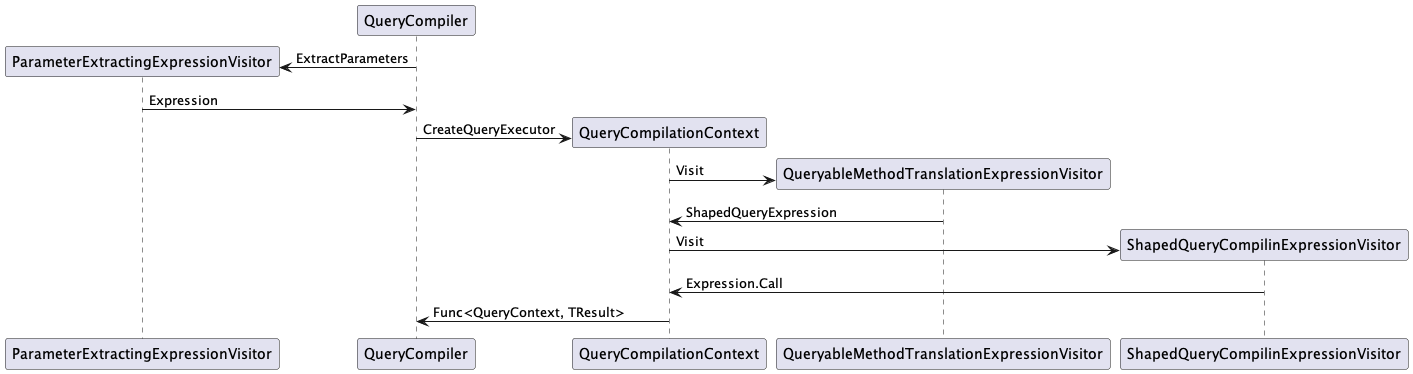
\includegraphics[width=\textheight, angle=-90]{content/Translation Sequence.png}
    \caption{\texttt{QueryCompiler} compilation sequence}
    \label{fig:QueryCompilerSequence}
\end{figure}

\section{Execute a command and retrieve the result}

We will be using Neo4js official driver for .NET to execute the query. The result of any query
is returned using \texttt{IResultCursor} interface. This interface is somewhat similar to an asynchronous
enumerator, but it does not implement the \texttt{IAsyncEnumerable<T>} interface. The \texttt{IResultCursor} interface
declares methods as show on the \ref{fig:iresinterface} picture. We will have to adapt our code to use this interface.
We are going to use these methods inside a proper implementation of \texttt{IAsyncEnumerable<T>}
interface.

\begin{figure}[H]
    \centering
    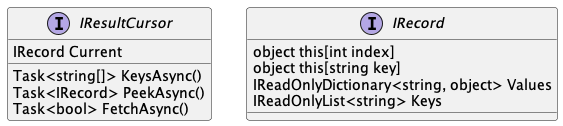
\includegraphics[width=0.7\textwidth]{content/IResultCursor.png}
    \caption{\texttt{IResultCursor} and \texttt{IRecord} interfaces}
    \label{fig:iresinterface}
\end{figure}

\section{Map the result of the query to an object}

Mapping result into an object is our last step. We already know from \ref{fig:iresinterface} class diagram,
that we can access an \texttt{IRecord} interface using \texttt{IResultCursor.Current} property.
This interface represents a single result of the query, which is defined in Cypher using \texttt{RETURN} clause.

Our mapper needs to read the result and correctly choose the right key from the values. IRecord is not a representation of a single node or relationship, but it is a representation of the \texttt{RETURN} clause, meaning that it contains all the values of the \texttt{RETURN} clause.
Mapper needs to know which key contains which entity and or value.

We can solve this issue by creating an extension method that will extend an \texttt{IRecord} interface and accept a \texttt{string} parameter defining an alias of value.
This method will return either a value or an entity.

\section{Summary}

In this chapter, we designed a solution for an \acrshort{ogm} library in .NET with LINQ to Cypher translation.
We started with defining six critical requirements that our library must solve and then went through each one of them and
proposed a solution for them.

We defined how we would handle creating a connection to the database using Neo4js official driver for .NET. Then we moved on
to the problem of mapping objects into graph structure using annotations and reflection. We also proposed a solution for mapping LINQ queries to
Cypher queries. At the end of this chapter, we went through the process of executing and mapping the Cypher query and its result back into objects.

With this design, we should have all that we need to successfully implement \acrshort{ogm} library for .NET with LINQ to Cypher translation.


\chapter {Implementation of proof-of-concept}

With the solution analysis done, we can now start implementing proof-of-concept.
Before we start the implementation, we should define the goals we want to accomplish in the proof-of-concept.
These are the goals:
\begin{itemize}
    \item {Create or update nodes in a database}
    \item {Map LINQ to Cypher}
\end{itemize}

The main tools used are Visual Studio Code with multiple plugins like Copilot and \CS\ extension, which provides an IntelliSense.
Github is used as VCS. Code is available at this URL \url{https://github.com/TomStary/dotnet-neo4j-ogm} or in the appendix of this thesis.

To create a new project, we will use the following command in the terminal application: \texttt{dotnet new classlib} with parameters for the name of the project and others.
We also want to separate tests from the source code of the library, so we employ a file structure like this \ref{ref:fileStructure}.

\begin{figure}[H]
    \dirtree{%
        .1 dotnet-neo4j-ogm.
        .2 src.
        .3 {Neo4j.OGM}.
        .2 tests.
        .3 {Neo4j.OGM}.
        .2 {.gitignore} .
        .2 {Neo4j.OGM.sln}.
    }
    \caption{File structure}
    \label{ref:fileStructure}
\end{figure}

With the file structure prepared, we can begin our implementation. During the development of this
library, we will use \acrfull{tdd}. We will not go deep into this approach in this chapter,
as it will be described in the next chapter, but keep in mind that during development, \acrshort{tdd} was used as it is an excellent way to write and test libraries.

\section {Common infrastructure}

If we want to achieve set goals for proof-of-concept, we will need a common infrastructure like the implementation of \texttt{ISession} interface.
This interface can be described as an entry point for all of our operations with the database. It will handle both saving entities and creating DbSet
instances, which can be used to query over entities using LINQ.

For the session to work properly, we need to have a few things:

\begin{itemize}
    \item connection to the database
    \item domain metadata
\end{itemize}

The connection to a database and domain metadata can be acquired from the session's constructor or elsewhere. However,
the best solution is to use \texttt{SessionFactory} instead. Using a factory has many benefits. The client's code will not be responsible for
creating a connection to the database for each session instance. It will also have precalculated domain metadata. Another benefit is
that it will be possible to hide the concrete implementation of \texttt{ISession} interface.

Implementation of \texttt{SessionFactory} is simple, we create a class with constructor accepts three parameters:
\begin{itemize}
    \item {\texttt{string connectionString} - contains connection string to the database}
    \item {\texttt{IAuthToken token} - token created by \texttt{AuthTokens} class from Neo4j drivers library, used to authenticate connections to the database}
    \item {\texttt{params Assembly[] assemblies} - assemblies containing domain models}
\end{itemize}
Using the first two parameters, we can create \texttt{IDriver} instance, which will be used to create session instances. The third parameter is special
because the type of the parameter is prefixed with keyword \texttt{params}. It means we can call the constructor with as many instances of \texttt{Assembly} as we want
(we are limited only by language itself, which has a cap at $2^{14}$ parameters). From \CS\ documentation:
"No additional parameters are permitted after the \texttt{params} keyword in a method declaration, and only one params keyword is permitted in a method declaration." \cite{billwagner_params_nodate}

The assemblies refer to where domain models are located; we need from the client's code information which assemblies to scan using reflection to pick up classes
representing nodes and relationships. We need this data for the correct graph analysis during saving operations.

\subsection {Building metadata}

We described the importance of metadata, but how are we going to obtain them. We already have assemblies from client's code, that should contain
the domain model. We use these assemblies in \texttt{MetaData} class constructor. Here is an actual implementation of \texttt{MetaData} constructor:

\begin{listing}[H]
    \begin{minted}[
 frame=lines,
 framesep=2mm,
 baselinestretch=1,
 bgcolor=LightGray,
 linenos,
 breaklines
 ] {csharp}
/// <summary>
/// MetaData constructor.
/// </summary>
/// <param name="assemblies">Assemblies containing domain model.</param>
internal MetaData(params Assembly[] assemblies)
{
 _domainInfo = new DomainInfo(assemblies);
 Schema = new SchemaBuilder(_domainInfo).Build();
}
 \end{minted}
    \caption{\texttt{MetaData} constructor}
    \label{code:metadataconstructor}
\end{listing}

We can now see how are the assemblies passed to the \texttt{DomainInfo} constructor, inside this class, we going through all the assemblies
and scanning all classes obtained by the \texttt{Assembly.GetType} method. This method return an array of \texttt{Type} objects representing
all the types in the assembly. We can then check each \texttt{Type} if it has an annotation for the node or relationship. We check this by using
our custom extension methods for \texttt{Type}, \texttt{HasNodeAttribute} and \texttt{HasRelationshipEntityAttribute}. If the type has the annotation,
we are going to add it to the right dictionary, which will be used during building the schema. We can see how this is done in the following code:

\begin{listing}[H]
    \begin{minted}[
 frame=lines,
 framesep=2mm,
 baselinestretch=1,
 bgcolor=LightGray,
 linenos,
 breaklines
 ] {csharp}
/// <summary>
/// Check if given <see cref="Type" does have the <see cref="NodeAttribute"> applied as custom attribute.
/// </summary>
internal static bool HasNodeAttribute(this Type type)
 => type.GetCustomAttributes().Any(attribute => attribute is NodeAttribute);

/// <summary>
/// Check if given <see cref="Type" does have the <see cref="RelationshipEntityAttribute"> applied as custom attribute.
/// </summary>
internal static bool HasRelationshipEntityAttribute(this Type type)
 => type.GetCustomAttributes().Any(attribute => attribute is RelationshipEntityAttribute);
 \end{minted}
    \caption{\texttt{HasNodeAttribute} and \texttt{HasRelationshipEntityAttribute} extension methods}
    \label{code:typeextensions}
\end{listing}

\subsection{\texttt{inline} keyword}

Keen reader might caught it up, but in last two code examples \ref{code:metadataconstructor} and \ref{code:typeextensions} we used the keyword \texttt{internal}
as an access modifier to the defined methods. This access modifier makes methods, classes, and properties available only inside the assembly. More on this subject
can be read at the official documentation of \CS\ language, URL: \url{https://docs.microsoft.com/en-us/dotnet/csharp/language-reference/keywords/internal}.

\subsection {Building schema}

Building schema is the last step in creating metadata for the client's domain model.
We use \texttt{SchemaBuilder} class to build the schema. We need to pass the \texttt{DomainInfo} instance to the \texttt{SchemaBuilder} constructor.
At the start we create new \texttt{Schema} instance, which is our concrete implementation of \texttt{ISchema} interface.

\texttt{SchemaBuilder.Build} method is responsible for building the schema. It does that by iterating over nodes and relationships and adding them to \texttt{Schema} instance
using \texttt{ISchema.AddNode} and \texttt{ISchema.AddRelationship} methods. The resulting schema is then returned.

We now have both schema and driver for creating the session. We will store both of them inside \texttt{SessionFactory} instance
and use them every time the session is created. To help client's code to manage instances of \texttt{SessionFactory} we will create an extension
of \texttt{IServiceCollection} which is a component of .NET responsible for managing the \acrfull{dic}. The lifetime of the \texttt{SessionFactory} is
a singleton, meaning that only one instance will be created during the runtime of the application. The extension implementation is shown here \ref{code:collectionextension}.

\begin{listing}[H]
    \begin{minted}[
 frame=lines,
 framesep=2mm,
 baselinestretch=1,
 bgcolor=LightGray,
 linenos,
 breaklines
 ] {csharp}
/// <summary>
/// Try and register the Neo4j OGM services in the DI container.
/// </summary>
public static IServiceCollection AddNeo4jOGMFactory(
 this IServiceCollection serviceCollection,
 string connectionString,
 IAuthToken authToken,
 params Assembly[] assemblies
 )
{
 serviceCollection.TryAddSingleton(
 new SessionFactory(connectionString, authToken, assemblies));
 return serviceCollection;
}
 \end{minted}
    \caption{\texttt{IServiceCollection} extension method}
    \label{code:collectionextension}
\end{listing}

With this extension method done, we have finished the common infrastructure, and we can now go and start implementing our
goals from the beginning of this chapter.

\section{Create or update nodes in a database}

\begin{listing}[H]
    \begin{minted}[
 frame=lines,
 framesep=2mm,
 baselinestretch=1,
 bgcolor=LightGray,
 linenos,
 breaklines
 ] {csharp}
/// <summary>
/// Save entity or list of entities to the database.
/// </summary>
public async Task SaveAsync<TEntity>(TEntity entity) where TEntity : class
{
 CheckDisposed();

 // tranform entity/entities into array
 IEnumerable<TEntity> objects;
 if (typeof(IEnumerable).IsAssignableFrom(entity.GetType()))
 {
 objects = (IEnumerable<TEntity>)entity;
 }
 else
 {
 objects = new[] { entity };
 }

 // map objects into a graph and creates statements
 foreach (var item in objects)
 {
 _entityGraphMapper.Map(item, -1);
 }

 // execute statements
 await ExecuteSave(_entityGraphMapper.CompilerContext());
}
 \end{minted}
    \caption{Internal implementation of save operation}
    \label{code:saveimpl}
\end{listing}

From the snippet above \ref{code:saveimpl} is an actual implementation of the save operation inside \texttt{ISession} concrete implementation.
We are going to use the \texttt{EntityGraphMapper} class to map the entity/entities into a structure that will be translated into
\texttt{IStatement} objects which represent statements that will be executed in the database. During mapping, we will also note the relationships between nodes
using information from \texttt{MetaData} object we built for this purpose. This whole concept is borrowed from
the official implementation of the Neo4j-\acrshort{ogm} library for Java.

\subsection{\texttt{EntityGraphMapper}}

The \texttt{EntityGraphMapper} is responsible for mapping the entities that will be translated into Cypher, as was stated in the paragraph before.
The resulting structure of this translation is saved inside a compiler context. The compiler context is a container for all the information
used during mapping and generating Cypher queries. It tracks visited nodes as well as visited relationships.

Inside the \texttt{ICompilerContext} is saved the instance of compiler, in this case it is \texttt{IMultiStatementCypherCompiler},
which is responsible for generating create and update Cypher queries. This compiler is used inside the\linebreak\texttt{Session.ExecuteSave} method.

\subsection{\texttt{IMultiStatementCypherCompiler}}

\begin{listing}[H]
    \begin{minted}[
 frame=lines,
 framesep=2mm,
 baselinestretch=1,
 bgcolor=LightGray,
 linenos,
 breaklines
 ] {csharp}
public interface IMultiStatementCypherCompiler
{
 CompilerContext Context { get; }
 NodeBuilder CreateNode(long id);
 IEnumerable<IStatement> CreateNodesStatements();
 NodeBuilder ExistingNode(long id);
 RelationshipBuilder ExistingRelationship(long relId, string type);
 IEnumerable<IStatement> GetAllStatements();
 bool HasStatementDependentOnNewNode();
 RelationshipBuilder NewRelationship(string type);
 RelationshipBuilder NewRelationship(string type, bool mapBothDirections);
 void UseStatementFactory(IStatementFactory statementFactory);
}
 \end{minted}
    \caption{\texttt{IMultiStatementCypherCompiler} interface}
    \label{code:IMultiStatementCypherCompiler}
\end{listing}

This interface defines a set of methods needed for preparing and generating \texttt{IStatement} instances that will then be executed on the database.
The \texttt{NodeBuilder} and \texttt{RelationshipBuilder} classes are what used inside\linebreak\texttt{EntityGraphMapper} and are the building blocks for
\texttt{IStatement} instances.

\subsection{\texttt{IStatement}}

The \texttt{IStatement} was mentioned multiple times. It is a simple wrapper around a string containing the Cypher query and dictionary of parameters
used in the query. These two values can then be used to generate \texttt{Query} object from Neo4j.Driver library. \texttt{Query} is used by
Neo4j.Driver in their transaction implementation.

\section{Mapping LINQ to Cypher}

The process of mapping LINQ to Cypher can be divided into these steps:
\begin{itemize}
    \item {prepare LINQ query}
    \item {map LINQ to our expression tree}
    \item {map our expression tree into Cypher}
    \item {map result from database into result object.}
\end{itemize}
We will look at each step and show some of the implementations.

\subsection{Prepare LINQ query}

Before we translate the query, we have to prepare our LINQ query. Preparation starts with the definition of the asynchronous method in the \texttt{DbSet<T>} class
or the \texttt{IQueryable<T>} extension of an asynchronous method. The best example of this definition would be method \texttt{FindAsync} as it is defined
in the \texttt{DbSet<T>} class, but it also uses an extension method for \texttt{IQueryable<T>} interface. The reason behind using asynchronous methods is
the implementation of \texttt{IDriver} which has only asynchronous methods for working with transactions.

Apart from the checks of the key values, the method will also create a lambda expression that will be translated into the \texttt{WHERE} statement
in the Cypher query. This lambda expression is then passed to the \texttt{FirstOrDefaultAsync} method, which is an extension of the \texttt{IQueryable<T>} interface
as we discussed above. The example below \ref{code:dbSetFindAsync} shows the exact implementation of the \texttt{DbSet<T>.FindAsync} method.
Inside the extension method of\linebreak\texttt{FirstOrDefaultAsync}, we are calling the \texttt{IAsyncQueryProvider.ExecuteAsync<T>} method. This method
is responsible for translation and execution of the query.

\begin{listing}[H]
    \begin{minted}[
 frame=lines,
 framesep=2mm,
 baselinestretch=1,
 bgcolor=LightGray,
 linenos,
 breaklines
 ] {csharp}
public virtual Task<TEntity?> FindAsync(params object?[]? keyValues)
{
 if (keyValues == null
 || keyValues.Any(key => key == null))
 {
 return Task.FromResult<TEntity?>(default);
 }

 var keyProperties = typeof(TEntity).GetProperties()
 .Where(property => property.GetCustomAttribute<KeyAttribute>() != null)
 .ToArray();

 if (keyProperties.Length != keyValues.Length)
 {
 throw new ArgumentException("Incorrect number of key values");
 }

 return this.FirstOrDefaultAsync(BuildLambda(keyProperties, new ValueBuffer(keyValues)));
}
\end{minted}
    \caption{\texttt{DbSet<T>.FindAsync} implementation}
    \label{code:dbSetFindAsync}
\end{listing}

\subsection{Expression visitors}

Our goal is to create a custom expression tree that would copy a Cypher with additional information about the mapping of the result.

First of all, we will introduce such classes to which we want to translate our LINQ expression tree \ref{fig:cypherexpression}.

\begin{figure}[H]
    \centering
    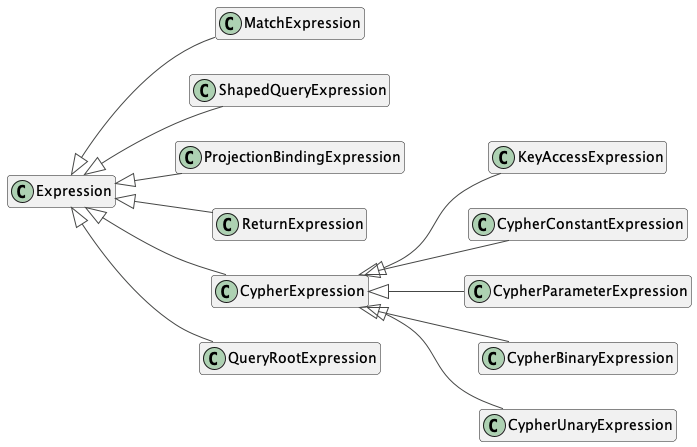
\includegraphics[width=\textwidth]{content/Cypher Expressions.png}
    \caption{Custom classes for translating LINQ expression tree}
    \label{fig:cypherexpression}
\end{figure}

To translate LINQ query to our custom expression tree, we will use the \texttt{QueryableMethodTranslationExpressionVisitor} class.
This class implements the \texttt{ExpressionVisitor} abstract class from LINQ. Our query is starts as \texttt{QueryRootExpression} which is
translated into \texttt{ShapedQueryExpression}. The \texttt{ShapedQueryExpression} contains the \texttt{MatchExpression} and\linebreak\texttt{EntityShaperExpression}
expression. This translation is done inside\linebreak\texttt{VisitExtension} method which is called for each expression marked with \texttt{ExpressionType.Extension}
as their \texttt{NodeType} property.

To set up \texttt{MatchExpression}, we are using a method \texttt{VisitMethodCall} which visits the children of the \texttt{MethodCallExpression}.
This method translates calls like \texttt{FirstOrDefault} from LINQ library. Inside this method the \texttt{WHERE} clause is translated as well
as \texttt{MatchExpression} other properties like\linebreak\texttt{MatchPattern.Limit}. Also the \texttt{ReturnExpression} is created inside this method.

The result of \texttt{Visit} method is a \texttt{ShapedQueryExpression} which contains the \texttt{MatchExpression}
with \texttt{ReturnExpression} and other predicates and expressions. This expression is now ready to be translated into Cypher query.

The visitor responsible for the actual translation to Cypher is\linebreak\texttt{CypherExpressionVisitor}. Inside this expression visitor,
we declare methods that corresponds with our custom classes, like \texttt{VisitCypherBinary} or \texttt{VisitMatch}. Each of these methods translates part of the expression
tree into a Cypher query. When the translation is done, the generated query is used in our custom enumerator, which enumerates the result from the database. This enumerator
is implemented inside \texttt{QueryingEnumerable<T>} class.

With the enumerator done, and the query generated, we need to execute our custom expression tree to get the result we want. To do this, we will use another visitor. In this case, this visitor needs to visit our\linebreak\texttt{ShapedQueryExpression} and create a right call that enumerates and returns the result.
The name of the class is\linebreak\texttt{ShapedQueryCompilingExpressionVisitor} and it checks if the result should be resulting in a single value or collection.
Inside, this visitor has also defined a custom lambda function, which will take the insides of\linebreak\texttt{ProjectionBindingExpression} and translate them to our result object.

\section{Summary}

This chapter was about implementing the library we designed in the chapter before. We described the structure of our project and then implemented
two critical goals of our proof-of-concept. With the first goal, we implemented the save operation for entities. We used metadata with information about graph
schema to properly create nodes and relationships. The second goal was mapping LINQ to Cypher query and extracting results from the database structure; we had to implement our own expressions structure to transform the expression tree so that we would be able to translate it to Cypher query.




\chapter {Test-driven development}

In the implementation chapter, we mentioned that tests were written during implementation and that the \acrshort{tdd} technique was used. "Test-driven development is a software development approach in which test cases are developed to specify
and validate what the code will do." \cite{hamilton_what_2020} What this means to us is that before the implementation of
our library, we should write a set of tests for our public \acrshort{api}. In this chapter, we will focus on implementing the tests
and some base principles of test-driven development and testing in general.

To write tests we need a framework that will help us write these tests. In .NET there are number of test frameworks that we can use, here is a list of
the most used ones:

\begin{itemize}
    \item {MSTest - Microsoft original test framework}
    \item {NUnit - Originaly ported from JUnit \cite{noauthor_nunitorg_nodate}}
    \item {xUnit - Created by author of the NUnit v2 \cite{noauthor_home_nodate}}
\end{itemize}

Per the author's experience, we will use the xUnit framework, but this type of testing is available in any of these frameworks.

.NET \acrshort{cli} tool has a template for xUnit project available under command \texttt{dotnet new xunit}. This command will
prepare a project with dependencies for xUnit and Microsoft.NET.Test.Sdk packages. It will also configure runners and coverlet.collector for collecting
code coverage.

\section{More information about \acrshort{tdd}}

Test-driven development can be summed up using an activity diagram. At the start of the development, we write down all the tests that we need to cover our code, and then we start with the implementation of the library. We refactor our code; for example, we mode code from one method into multiple methods and even classes.
After refactoring is done, we check our tests and write new ones.

\begin{figure}[H]
    \centering
    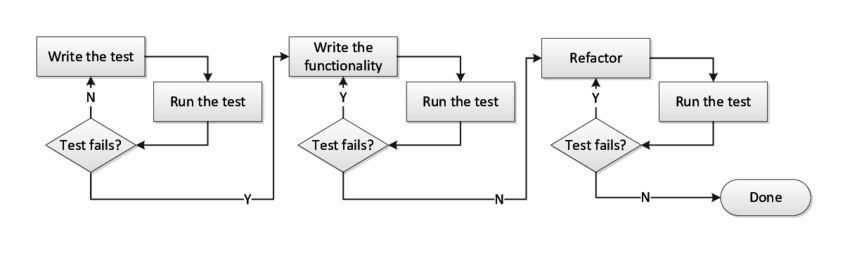
\includegraphics[width=\textwidth]{content/Test-Driven-Development-activities.png}
    \caption{Test-driven development diagram \cite{noauthor_continuous_2013}}
    \label{fig:tddDiagram}
\end{figure}

Using this approach has many benefits. One of them is complete code coverage of our code, which means that tests should cover every line. We will use the coverlet tool to calculate the coverage, which is a cross-platform coverage framework for .NET. \cite{noauthor_coverlet_2022} It supports multiple output
formats, but for our case, we will use \texttt{lcov} format, which can be then loaded by extension in Visual Studio Code and display coverage information directly in files.
We can also generate a report of the coverage using these commands.
\begin{itemize}
    \item {\texttt{dotnet test \textbackslash\\
              /p:CollectCoverage=true \textbackslash\\/p:CoverletOutput=../../lcov.info \textbackslash\\/p:CoverletOutputFormat=lcov}}
    \item {\texttt{genhtml lcov.info -o ./CoveragerReport/}}
\end{itemize}
The first command is to execute tests and generate \texttt{lcov.info} file, which contains coverage information. This file is also used by extension for Visual Studio Code
named Coverage Gutters.
Second command is to generate html report from \texttt{lcov.info} file.

Here \ref{fig:report} is an example of the report from this project.

\begin{figure}[H]
    \centering
    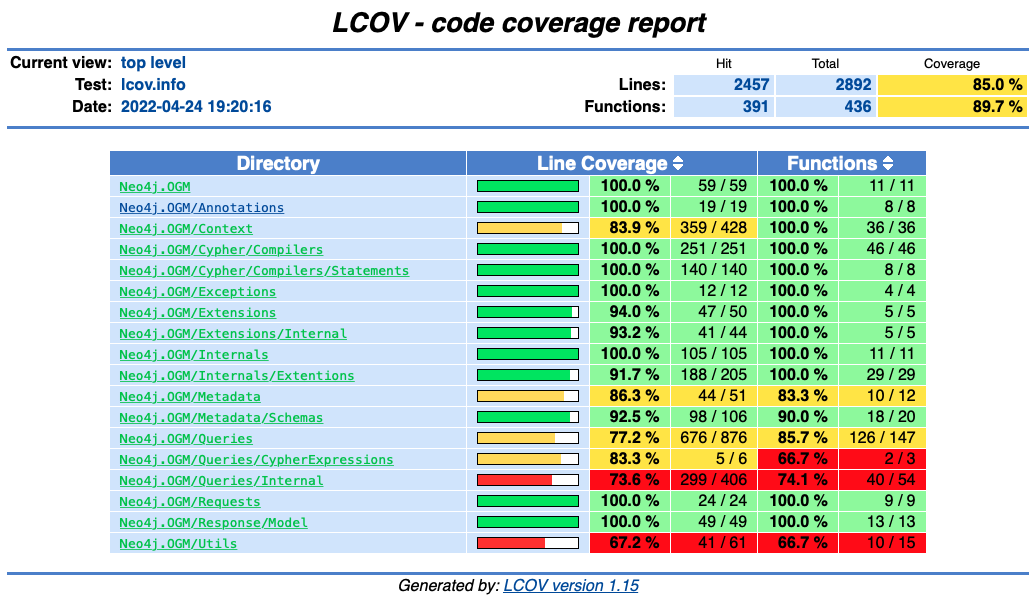
\includegraphics[width=\textwidth]{content/coverage_report.png}
    \caption{Example of the report}
    \label{fig:report}
\end{figure}
\todo[inline]{Better coverage report image}

\section{\texttt{SessionFactory} tests}

We will start with testing \texttt{SessionFactory} as it is the entry point to use our library. Tests will be simple,
we want to test that \texttt{SessionFactory.Create} return an instance of \texttt{ISession} and that if the configuration
set on creating \texttt{SessionFactory} is invalid, that proper exception will be thrown.

\subsection{Mocking}

When writing tests for \texttt{SessionFactory}, we encountered a problem with sending assemblies containing our domain model to the \texttt{SessionFactory}
constructor. We want these assemblies to be mocked.

What is mocking? "Mocking is a process used in unit testing when the unit being tested has external dependencies.
The purpose of mocking is to isolate and focus on the code being tested and not on the behavior or state of external dependencies.
In mocking, the dependencies are replaced by closely controlled replacements
objects that simulate the behavior of the real ones." \cite{noauthor_mocking_nodate}

For our case, we will use a library for .NET called Moq, which is available as a NuGet package. More information about this package can
be found at \url{https://github.com/moq/moq4}.

With sample \ref{code:SessionFactoryCreateTest} of one of the tests for \texttt{SessionFactory.Create}, we can see how we are applying mocking in this test.
In the code sample \ref{code:SessionFactoryCreateTest}, we are firstly creating a mock of \texttt{Assembly} class, and then we also are creating a fake result for
one of the methods in the \texttt{Assembly} class. This method is used internally inside the library, and we need to define our result to be able to inject the suitable
array of classes against which we want to test.

\begin{listing}[H]
    \begin{minted}[
 frame=lines,
 framesep=2mm,
 baselinestretch=1,
 bgcolor=LightGray,
 linenos,
 breaklines
 ] {csharp}
 public void CreateTestResultOk()
 {
 var assembly = new Moq.Mock<Assembly>();
 assembly.Setup(a => a.GetTypes()).Returns(new[] { typeof(Person), typeof(Post) });

 var sessionFactory = new SessionFactory(
 "connectionString",
 AuthTokens.Basic("username", "password"),
 assembly.Object);

 var session = sessionFactory.Create();

 Assert.NotNull(session);
 Assert.IsAssignableFrom<ISession>(session);
 }
 \end{minted}
    \caption{Example of \texttt{SessionFactory} test with mocking of \texttt{Assembly} object}
    \label{code:SessionFactoryCreateTest}
\end{listing}

\section{Testing internal classes and methods}

In our library, we are using a keyword \texttt{internal} which hides classes, methods, or properties from other assemblies,
but because we also want to test these classes and their methods, we need to expose them. Exposing \texttt{internal} is possible
with a slight change in the project file. We need to add this \ref{code:csprojinternal} to the library project file, and our tests will be able to access every internal
class and method.

\begin{listing}[H]
    \begin{minted}[
 frame=lines,
 framesep=2mm,
 baselinestretch=1,
 bgcolor=LightGray,
 linenos,
 breaklines
 ] {xml}
<ItemGroup>
 <AssemblyAttribute
 Include="System.Runtime.CompilerServices.InternalsVisibleTo">
 <_Parameter1>Neo4j.OGM.Tests</_Parameter1>
 </AssemblyAttribute>
</ItemGroup>
 \end{minted}
    \caption{Edit of \texttt{Neo4j.OGM.csproj} to access internal classes and methods inside test project}
    \label{code:csprojinternal}
\end{listing}

Using this alteration of the \texttt{Neo4j.OGM.csproj} to access internal classes and methods inside the test project,
we can now prepare a test for internal classes and methods.

\section {Setup and cleanup}

Some of our tests will need to prepare data and mocks. We call this step of tests a setup step. nUnit for example, uses annotations
to mark cleanup (\texttt{TearDownAttribute}) and setup (\texttt{SetUpAttribute}) methods. However, in xUnit, we are using only constructors and \texttt{IDisposable}
interface for setup and cleanup, respectively. This approach has a limitation in not being able to perform asynchronous operations safely,
but xUnit has a solution for this too. \texttt{IAsyncLifetime} is an interface from xUnit that provides the means to perform setup and cleanup
methods asynchronously.

Apart from setup and cleanup methods, xUnit also offers an ability to share context between tests, either in one class or across multiple classes
using class fixtures or collection fixtures, more on this subject can be found in the official documentation of the xUnit framework.

\section {Summary}

We have now described all the parts of our testing, tests are ready, and we can start with the cycle of implementation and testing
as described in \acrshort{tdd}. This chapter was put after the implementation for clarity reasons.

\chapter {Deployment}

This chapter will focus on deploying our library to the NuGet repository, GitHub actions, and setting up our repository to attract more contributors.

\section {NuGet repository}

The primary source of packages for .NET applications is \url{https://www.nuget.org}.
Every developer can upload their packages to this repository, and anyone can then search and download packages from this feed.

Before uploading our library to the NuGet repository, we need to set our project properly.
We can find out everything we need on the ``Package authoring best practices'' page in Microsoft's documentation. \cite{gill_package_2022}

From the documentation page \cite{gill_package_2022} we know the properperties we need to set, here is their list:

\begin{itemize}
    \item \texttt{PackageId}: name of the package, which will be used in NuGet repository.
    \item \texttt{Authors}: list of authors of the package.
    \item \texttt{Description}: description of the package.
    \item \texttt{Copyright}: copyright details of the package.
\end{itemize}

With these properties set, we can now create a registration on NuGet and create an \acrshort{api} key for uploading packages using the command line.
There is also a possibility to upload a package using the form on the NuGet page itself, but we want to have this process automated using GitHub actions.

\section{GitHub actions}

GitHub actions is a tool for automation of the \acrfull{cicd} process, which allows us to automate tasks like running tests, checking build status, and publishing packages.
It is also possible to run tasks on a schedule, like creating nightly builds of our application or library.

We created three different workflows for our library, each for a different operation in \acrshort{vcs}. The operations are:
\begin{itemize}
    \item push --- every push of new commits onto the GitHub server will trigger this workflow.
    \item pull request --- every new pull request to the main branch or update to the pull request will trigger this workflow.
    \item release --- each new tag in the main branch will trigger this workflow.
\end{itemize}
These workflows will check our library's build status and the execution of the tests we wrote for our library.
In the case of release, the workflow will also create a new version of our library and publish it to the NuGet repository.

Workflows also offer us the possibility for static analysis of the codebase. This analysis is helpful as it scans code for common mistakes and potential vulnerabilities.
The static analysis is not used in this project, but it is something we can use in the future.

\section{Setting up repository}

One of our main goals with this library is that it will be easy for the community to expand our solution and report any issues with our library.
For this reason, we will follow the GitHub community standards. These standards should ensure that anyone can contribute to our project.
The list of community standards:
\begin{itemize}
    \item {Description}
    \item {README}
    \item {Code of conduct}
    \item {License}
    \item {Issue templates}
    \item {Pull request templates}
\end{itemize}

Some of these steps can be generated on GitHub using their templates, like license and code of conduct.
Others have to be defined by us. In the repository is a folder called \texttt{.github} which contains all the files that we need to set up, except for README and license files which are in the root folder of the repository.

\section{Summary}

With the community standards set up, we have everything we need to release our library.
Our repository on the GitHub server can be made public, and we can release our library to the NuGet repository.
We can now plan the following steps to finish our library.


\chapter{Evaluation of the project}

We will now evaluate our project, we can divide this evalutation into three parts.

The first part is the evaluation of our design of the OGM library. The design was inspired by both the Ne4oj-\acrshort{ogm} for Java implementation and the Entity Framework.
The result is a working design of the library, but with some limitations which should be addressed in future development, namely the lack of the change tracker.

The second part of this evaluation is the implementation of a proof-of-concept for the design.
We set two goals for the proof-of-concept:
\begin{itemize}
    \item {Create or update nodes in a database}
    \item {Map LINQ to Cypher}
\end{itemize}
These two goals we achieved but during the implementation we noticed the missing change tracker, which severely limits the functionality of the library.

The first goal was achieved, with the help of already existing implementation in Java. Parts of the code were translated from Java to \CS\ with some changes to reflect the best practices.
This allowed us to quickly develop the save mechanism for our library, although it was not the best solution.
The problem with this solution is the different architecture of the library in the Java and .NET.
In the .NET, we would greatly benefit from the ability to use dependency injection, which is not used in Java implementation.
One thing we could also borrow from the Entity Framework is change tracker, this component of the Entity Framework gives us ability to track changes and save only the changes, it is also implemented using LINQ extensions.
The extensions would be easy to implement, because we already have some basic functionality in the library.

The second goal was to use the LINQ to create Cypher queries for the Neo4j database.
This goal was far more challinging to acomplish then the first one.
We had to remap original expression tree into a new one, that could be translated into Cypher query and with the use of Neo4j driver for .NET executed and mapped to the objects.
We acomplished this goal also with some limitations, but these limitations were more about the time and the size of the implementation itself than the problem with the design.
The only missing part for this goal is the ability to correctly map relationship between objects and agregation methods.


The third part of this evaluation is the projects setup for contributors.
This part is fully completed, we created a set of GitHub actions for our \acrshort{cicd}, prepared contributor's guide and release our library on NuGet repository feed.


\section{Next steps}

We will propose next steps for this library, and also document them in the repository using issues. The next steps should be the following:
\begin{itemize}
    \item {Implement the change tracker.}
    \item {Refactor internal classes to use dependency injection.}
    \item {Implement the save operation with the use of the change tracker.}
    \item {Implement the mapping of the objects using LINQ like it is done in the Entity Framework.}
\end{itemize}
With these steps done, we could release our library as production ready and could be used in commercial projects.

One other thing is missing for this project and that is proper user oriented documentation.
As this is a proof-of-concept, we did not create any documentation for the library, except for the \texttt{README} file.
However for the future development, there should be also a goal of creating proper documentation for the library.

The author of this publication will pursue the next steps to finish the project even after finishing this publication.

\bibliographystyle{iso690}
\bibliography{mybibliographyfile}

\setsecnumdepth{all}
\appendix

% \chapter{Acronyms}
\printglossaries
% \end{description}


\chapter{Contents of enclosed CD}

%change appropriately

\begin{figure}
    \dirtree{%
        .1 readme.txt\DTcomment{the file with CD contents description}.
        .1 exe\DTcomment{the directory with executables}.
        .1 src\DTcomment{the directory of source codes}.
        .2 wbdcm\DTcomment{implementation sources}.
        .2 thesis\DTcomment{the directory of \LaTeX{} source codes of the thesis}.
        .1 text\DTcomment{the thesis text directory}.
        .2 thesis.pdf\DTcomment{the thesis text in PDF format}.
        .2 thesis.ps\DTcomment{the thesis text in PS format}.
    }
\end{figure}

\end{document}
